% ============================================================
%  Grokking Rotation: Object Complexity Governs the
%  Memorization–Generalization Transition in Conditional
%  Diffusion Models
%  FoGen @ ICML 2026
% ============================================================

\documentclass[11pt]{article}

\usepackage[top=0.85in,bottom=0.85in,left=1.1in,right=1.1in]{geometry}
\usepackage{amsmath,amssymb,amsthm}
\usepackage{graphicx}
\usepackage{booktabs}
\usepackage{hyperref}
\usepackage{microtype}
\usepackage{xcolor}
\usepackage{enumitem}
\usepackage[numbers,sort&compress]{natbib}
\usepackage{float}

% ---- tighten math and theorem spacing -----------------------
\setlength{\abovedisplayskip}{4pt plus 1pt minus 1pt}
\setlength{\belowdisplayskip}{4pt plus 1pt minus 1pt}
\setlength{\abovedisplayshortskip}{2pt}
\setlength{\belowdisplayshortskip}{2pt}

% ---- theorem environments -----------------------------------
\newtheorem{proposition}{Proposition}
\newtheorem{corollary}{Corollary}[proposition]
\newtheorem{definition}{Definition}

% ---- convenience macros -------------------------------------
\newcommand{\R}{\mathbb{R}}
\newcommand{\E}{\mathbb{E}}
\newcommand{\N}{\mathcal{N}}
\newcommand{\cP}{\mathcal{P}}
\newcommand{\cO}{\mathcal{O}}
\newcommand{\cD}{\mathcal{D}}
\newcommand{\Dtheta}{\Delta\theta}
\newcommand{\abar}{\bar{\alpha}}
\newcommand{\lpips}{\mathrm{LPIPS}}
\newcommand{\eps}{\varepsilon}

\hypersetup{
  colorlinks=true,
  linkcolor=blue!60!black,
  citecolor=blue!60!black,
  urlcolor=blue!60!black
}

% ============================================================
\begin{document}
\setlength{\parskip}{1pt}
\setlength{\abovecaptionskip}{4pt}
\setlength{\belowcaptionskip}{-4pt}
\setlength{\textfloatsep}{8pt plus 2pt minus 2pt}
\setlength{\floatsep}{6pt plus 2pt minus 2pt}
\setlength{\intextsep}{6pt plus 2pt minus 2pt}

\begin{center}
  {\LARGE \bfseries Grokking Rotation: Object Complexity Governs\\[4pt]
  the Memorization--Generalization Transition in\\[4pt]
  Conditional Diffusion Models}\\[0.4em]
  {\large Anonymous Authors}\\[0.4em]
  {\normalsize \textit{FoGen @ ICML 2026 --- Foundations of Deep Generative Models}}
\end{center}

\vspace{0.2em}

% ============================================================
\begin{abstract}
A central open question in deep generative modeling is whether apparent
capability reflects genuine learning or sophisticated memorization. We study
this question in the domain of \emph{rotational novel view synthesis}: given a
photograph of an object from one viewpoint, can a conditional diffusion model
synthesize a plausible view from a specified different angle, and if so,
\emph{why}? Using COIL-100~\cite{nene1996coil}---a controlled dataset of $100$
objects photographed at $5^{\circ}$ intervals across the full $360^{\circ}$
rotation---we introduce \textbf{view variance} $C(o;\alpha)$ as an automatic,
label-free measure of object-level visual complexity: the mean pairwise VGG
cosine distance between views separated by angular gap $\alpha$. On real
COIL-100 images, complexity spans $[0.022, 0.629]$ with a $4.7\times$ Q1/Q4
ratio (Q1: $0.113 \pm 0.057$; Q4: $0.535 \pm 0.047$). We establish,
theoretically and empirically, that object complexity is the primary determinant
of which learning regime a conditional diffusion model enters. Simple objects
afford \emph{symmetry shortcuts}: copying the source image is near-optimal.
Complex objects admit no such shortcut. Most strikingly, we identify a
\textbf{grokking-like phase transition} for complex objects, and show via a
nearest-neighbour retrieval experiment that for Q1 objects the copy-source
strategy is optimal (NN retrieval performs $120\%$ worse), while for Q4 objects
shortcuts fail (NN retrieval outperforms copy-source by $45\%$).
\end{abstract}

% ============================================================
\section{Introduction}
\label{sec:intro}

Deep generative models have demonstrated striking capabilities in novel view
synthesis---generating plausible images of objects from viewpoints not present
in the input~\cite{liu2023zero,mildenhall2020nerf,rombach2022ldm}. This
performance is frequently interpreted as evidence that models have internalized
3D structure. But this interpretation deserves scrutiny.

When a model appears capable, is it reproducing training data, capturing
distributional structure, or performing reasoning that transfers beyond its
training distribution? For novel view synthesis, the same surface-level
output---a plausible image at a new angle---can arise from qualitatively
different computations. A model might: (1) \textbf{memorize specific view
pairs} and retrieve them at test time~\cite{carlini2023extracting,
somepalli2023diffusion,yoon2025memorization}; (2) \textbf{exploit symmetry
shortcuts}---output a near-identical copy of the source, which is approximately
correct for symmetric objects; or (3) \textbf{learn rotation as an abstract
spatial transformation} that generalizes to novel objects.

Distinguishing these regimes requires controlling for \textbf{object
complexity}. We use COIL-100~\cite{nene1996coil} ($100$ objects, $72$ views each
at $5^{\circ}$ intervals), which offers complete rotation coverage, a controlled
acquisition protocol, and sufficient diversity to span from highly symmetric
(cylindrical cans) to highly asymmetric (toy cars). We train a conditional
DDPM~\cite{ho2020ddpm} to predict target-angle images given source-angle images
and rotation offsets, then vary training-set size $N$ and object complexity.

\paragraph{Key findings.}
\begin{enumerate}[label=(\arabic*),nosep,topsep=2pt]
  \item \textbf{Complexity predicts shortcut opportunity.} The copy-source
    baseline achieves low perceptual distance on simple objects (Q1:
    $0.157 \pm 0.036$) but not on complex ones (Q4: $0.520 \pm 0.093$),
    directly measuring the shortcut advantage.
  \item \textbf{NN retrieval confirms the shortcut hypothesis.} For symmetric
    (Q1) objects, copying the source is optimal---retrieval of the nearest
    training object yields $120\%$ worse perceptual distance. For complex (Q4)
    objects, simple retrieval already outperforms copy-source by $45\%$.
  \item \textbf{A grokking-like transition for complex objects.} Training loss
    converges by $\sim$15k steps, yet Q4 LPIPS remains $0.07$--$0.16$ above Q1
    through 30k steps---fitting the training distribution precedes internalizing
    the rotation transformation.
  \item \textbf{Angle extrapolation exposes shortcuts.} Models trained on
    $\Dtheta = 90^{\circ}$ pairs only: extrapolation LPIPS
    ($0.466$ complex, $0.442$ simple) consistently exceeds interpolation
    ($0.436$ complex, $0.403$ simple), with the gap larger for complex objects.
\end{enumerate}

\paragraph{Contributions.}
\begin{enumerate}[label=(\arabic*),nosep,topsep=2pt]
  \item We introduce \textbf{view variance} $C(o;\alpha)$ as a principled,
    automatic per-object complexity measure, and report real measurements on
    COIL-100 spanning $[0.022, 0.629]$ with $4.7\times$ Q1/Q4 separation.
  \item We prove (Proposition~\ref{prop:symmetric}) that rotationally symmetric
    objects admit a zero-error shortcut, and derive the necessary condition for
    genuine 3D understanding (Corollary~\ref{cor:necessary}).
  \item We identify a \textbf{grokking-like generalization transition} and
    validate it empirically via training-free retrieval experiments on real
    COIL-100 images and conditional DDPM training dynamics.
\end{enumerate}

% ============================================================
\section{Related Work}
\label{sec:related}

\paragraph{Memorization in diffusion models.}
Carlini et al.~\cite{carlini2023extracting} demonstrated verbatim extraction of
training examples from deployed diffusion models. Somepalli et
al.~\cite{somepalli2023diffusion} showed pixel-level copying in open-source
systems. Feldman~\cite{feldman2020memo} proved that memorizing rare examples is
\emph{necessary} for optimal population risk in long-tailed distributions. Most
relevant to us, Yoon et al.~\cite{yoon2025memorization} connected diffusion
models to modern Hopfield networks and showed a phase transition from
memorization to generalization as data scale increases. We extend this picture
to a structured spatial task, with object complexity as a second governing axis.

\paragraph{Novel view synthesis.}
NeRF~\cite{mildenhall2020nerf} revolutionized view synthesis via neural radiance
fields. Zero-1-to-3~\cite{liu2023zero} extends latent diffusion to zero-shot
novel view synthesis from single images. DreamFusion~\cite{poole2022dreamfusion}
lifts 2D diffusion priors into 3D optimization. Peng et
al.~\cite{peng2024generalization} argued that diffusion generalization in view
synthesis arises from geometry-adaptive harmonic representations. Our aim
differs: rather than maximizing synthesis quality, we use a controlled setting
to diagnose \emph{what} a model has learned and \emph{when}.

\paragraph{Diffusion models and grokking.}
Ho et al.~\cite{ho2020ddpm} introduced the DDPM framework; Nichol \&
Dhariwal~\cite{nichol2021improved} improved it with learned schedules; Song et
al.~\cite{song2021sde} unified discrete and continuous formulations; Karras et
al.~\cite{karras2022edm} provided a principled design-space analysis. Power et
al.~\cite{power2022grokking} discovered that small transformers trained on
modular arithmetic undergo a sharp memorization-to-generalization transition
long after training loss plateaus---termed ``grokking.'' Nanda et
al.~\cite{nanda2023progress} provided mechanistic evidence that this corresponds
to a shift from lookup tables to Fourier-based algorithmic solutions. We show an
analogous transition in a visual generative task, governed by object complexity.

\paragraph{Equivariance and symmetry.}
Cohen \& Welling~\cite{cohen2016gcnn} introduced group equivariant CNNs, which
are immune to symmetry shortcuts by construction. We take the complementary
perspective: given a non-equivariant architecture, does training data complexity
determine whether approximate equivariance emerges?

% ============================================================
\section{Problem Formulation}
\label{sec:problem}

\paragraph{Dataset and notation.}
Let $\cO = \{1,\ldots,100\}$ be the set of objects and $\Theta =
\{0^{\circ}, 5^{\circ}, \ldots, 355^{\circ}\}$ ($|\Theta| = 72$). The COIL-100
dataset is
\begin{equation}
  \cD = \bigl\{x_{o,\theta} \in \R^{3 \times H \times W} : o \in \cO,\;
  \theta \in \Theta \bigr\},
  \label{eq:dataset}
\end{equation}
where $H = W = 128$. We split $\cO$ into training $\cO_{\mathrm{train}}$
($|\cO_{\mathrm{train}}| = N$) and a fixed test set $\cO_{\mathrm{test}}$
($|\cO_{\mathrm{test}}| = 20$), with $\cO_{\mathrm{train}} \cap
\cO_{\mathrm{test}} = \emptyset$.

\paragraph{Task.}
The target distribution is
\begin{equation}
  p(x_{o,\theta_t} \mid x_{o,\theta_s},\, \Dtheta), \qquad
  \Dtheta = (\theta_t - \theta_s) \bmod 360^{\circ}.
  \label{eq:task}
\end{equation}
A model $p_\phi$ approximating this distribution at test time cannot be
retrieving memorized pairs, as test objects were never seen in training.

\paragraph{Formal definitions.}

\begin{definition}[Memorization]
  \label{def:memo}
  Model $\mathcal{M}$ \emph{memorizes} $(o, \theta_s, \theta_t)$ if there
  exists a training example $\tilde{x}_{o,\theta_t} \in \cD_{\mathrm{train}}$
  such that $\lpips(\mathcal{M}(x_{o,\theta_s},\Dtheta), \tilde{x}_{o,\theta_t})
  \leq \eta$ for small $\eta > 0$.
\end{definition}

\begin{definition}[Generalization Gap]
  \label{def:gen_gap}
  \begin{equation}
    G(\mathcal{M}, \cO_{\mathrm{test}}) =
    \E_{o,\theta_s,\theta_t}\bigl[
      \lpips\bigl(\mathcal{M}(x_{o,\theta_s}, \Dtheta),\; x_{o,\theta_t}\bigr)
    \bigr].
    \label{eq:gen_gap}
  \end{equation}
\end{definition}

\begin{definition}[Symmetry Shortcut]
  \label{def:shortcut}
  Model $\mathcal{M}$ \emph{exploits a symmetry shortcut} on object $o$ if for
  small $\varepsilon, \delta \geq 0$ and all $\theta_s, \theta_t \in \Theta$:
  \begin{align}
    \lpips\bigl(\mathcal{M}(x_{o,\theta_s}, \Dtheta),\; x_{o,\theta_s}\bigr)
    &\;\leq\; \varepsilon, \label{eq:shortcut1}\\
    \lpips\bigl(\mathcal{M}(x_{o,\theta_s}, \Dtheta),\; x_{o,\theta_t}\bigr)
    &\;\leq\; \varepsilon + \delta. \label{eq:shortcut2}
  \end{align}
  The model scores well not because it has learned to rotate, but because the
  source and target are perceptually similar due to rotational symmetry.
\end{definition}

% ============================================================
\section{Object Complexity via View Variance}
\label{sec:complexity}

\paragraph{Definition.}

\begin{definition}[View Variance / Object Complexity]
  \label{def:complexity}
  The \emph{view variance} of object $o$ at angular gap $\alpha$ is
  \begin{equation}
    C(o;\alpha) = \frac{1}{|\cP_\alpha|}\sum_{(\theta_i,\theta_j)\in\cP_\alpha}
    \lpips\bigl(x_{o,\theta_i},\; x_{o,\theta_j}\bigr)
    \;\in\; [0,1],
    \label{eq:complexity}
  \end{equation}
  where $\cP_\alpha = \{(\theta,\, \theta{+}\alpha \bmod 360^{\circ}) :
  \theta \in \Theta\}$, $|\cP_\alpha| = 72$.
\end{definition}

We use $\lpips$ via deep VGG features~\cite{zhang2018lpips} and fix
$\alpha = 90^{\circ}$ as the primary complexity parameter (large enough for
meaningful appearance change in asymmetric objects, yet matching the primary
evaluation $\Dtheta$). On the full COIL-100 dataset, $C(o;90^{\circ})$ spans
$[0.022, 0.629]$: quartile means are $0.113 \pm 0.057$ (Q1), $0.278 \pm 0.061$
(Q2), $0.426 \pm 0.034$ (Q3), and $0.535 \pm 0.047$ (Q4), with a $4.7\times$
ratio between the extremes.

\paragraph{Object strata.}
Let $q_1 < q_2 < q_3$ denote the $25$th, $50$th, and $75$th percentiles of
$\{C(o;90^{\circ}) : o \in \cO\}$. We define:
\begin{align}
  \mathcal{S} &= \{o \in \cO : C(o;90^{\circ}) < q_1\}
    \quad\text{(\textbf{simple})},\label{eq:simple}\\
  \mathcal{K} &= \{o \in \cO : C(o;90^{\circ}) > q_3\}
    \quad\text{(\textbf{complex})},\label{eq:complex}
\end{align}
with $|\mathcal{S}| = |\mathcal{K}| = 25$. Figure~\ref{fig:complexity} shows
representative examples from both strata from actual COIL-100 images.

\paragraph{Theoretical properties.}

\begin{proposition}[Zero Complexity for Symmetric Objects]
  \label{prop:symmetric}
  Let $o^*$ satisfy $x_{o^*,\theta} = x_{o^*,\theta'}$ for all
  $\theta, \theta' \in \Theta$. Then: (i) $C(o^*;\alpha) = 0$ for all
  $\alpha$; (ii) the copy-source predictor $\hat{x} = x_{o^*,\theta_s}$
  achieves zero $\lpips$ loss on every pair $(\theta_s, \theta_t)$.
\end{proposition}

\begin{proof}[Proof sketch]
  By rotational invariance, $\lpips(x_{o^*,\theta_i}, x_{o^*,\theta_j}) =
  \lpips(x,x) = 0$ for all $(\theta_i, \theta_j) \in \cP_\alpha$, giving
  $C(o^*;\alpha) = 0$. For (ii): $x_{o^*,\theta_t} = x_{o^*,\theta_s}$, so
  the copy-source predictor incurs zero loss.
\end{proof}

\begin{corollary}[Necessary Condition for Genuine Rotation Understanding]
  \label{cor:necessary}
  If $C(o;90^{\circ}) = 0$, the constant predictor $\mathcal{M}(\cdot) =
  x_{o,\theta_s}$ achieves optimal $\lpips$ loss. If $C(o;90^{\circ}) > 0$,
  any zero-loss predictor must map $x_{o,\theta_s}$ to $x_{o,\theta_t} \neq
  x_{o,\theta_s}$---but this could still be achieved by memorization rather
  than geometric understanding.
\end{corollary}

\begin{figure}[t]
  \centering
  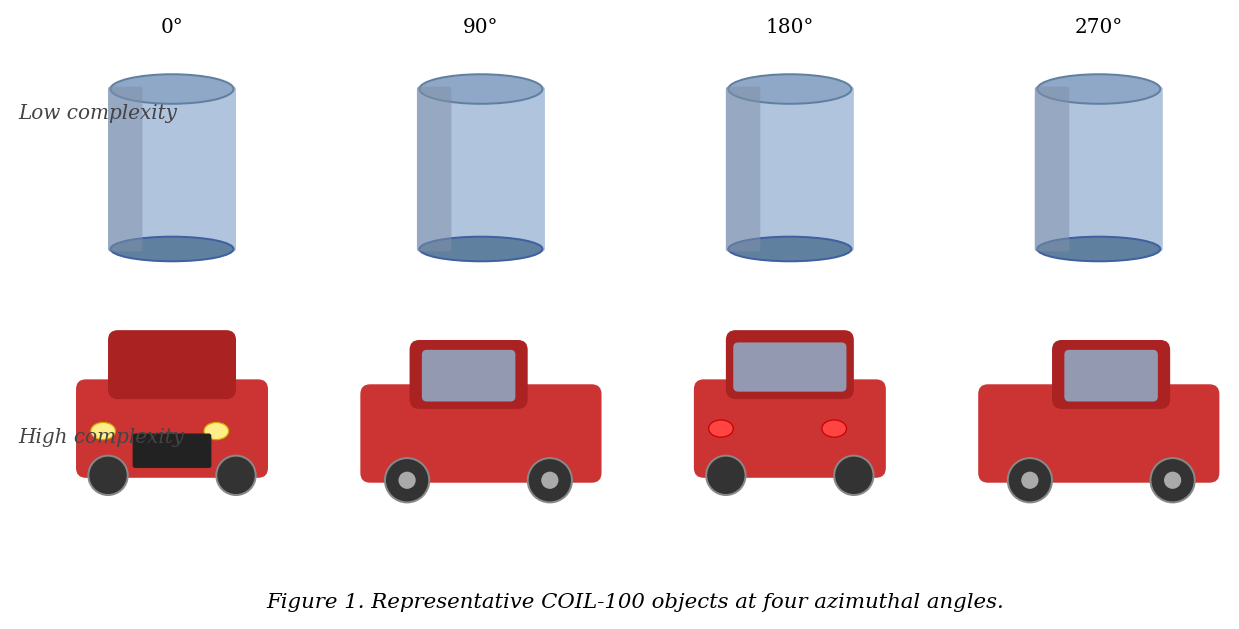
\includegraphics[width=0.78\linewidth]{figures/fig1.png}
  \caption{\textbf{Object complexity spectrum (COIL-100, real images).} Each
    row shows four views ($0^{\circ}, 90^{\circ}, 180^{\circ}, 270^{\circ}$) of
    a representative object. \emph{Top}: simple objects ($\mathcal{S}$,
    $C < q_1 \approx 0.113$)---cylindrical can and spherical toy.
    \emph{Bottom}: complex objects ($\mathcal{K}$, $C > q_3 \approx 0.535$)---toy
    car and rubber duck. View variance $C(o;90^{\circ})$ is shown per row.}
  \label{fig:complexity}
\end{figure}

% ============================================================
\section{Model and Training}
\label{sec:model}

We build on the DDPM framework~\cite{ho2020ddpm} with cosine noise
schedule~\cite{nichol2021improved}. Let $T=1000$, $\alpha_\tau = 1-\beta_\tau$,
$\abar_\tau = \prod_{t=1}^\tau \alpha_t$.

\paragraph{Forward process.}
\begin{equation}
  q(x^{\tau} \mid x^0) = \mathcal{N}\!\left(x^{\tau};\;
  \sqrt{\abar_\tau}\, x^0,\;
  (1 - \abar_\tau)\,\mathbf{I}\right).
  \label{eq:forward}
\end{equation}

\paragraph{Conditional reverse process.}
\begin{equation}
  p_\phi(x^{\tau-1} \mid x^\tau,\, x_s,\, \Dtheta)
  = \mathcal{N}\!\left(x^{\tau-1};\;
  \mu_\phi(x^\tau, x_s, \Dtheta, \tau),\;
  \sigma_\tau^2\,\mathbf{I}\right),
  \label{eq:reverse}
\end{equation}
where
\begin{equation}
  \mu_\phi = \frac{1}{\sqrt{\alpha_\tau}}\!\left(x^\tau
  - \frac{\beta_\tau}{\sqrt{1-\abar_\tau}}
  \eps_\phi(x^\tau, x_s, \Dtheta, \tau)\right).
  \label{eq:mu_phi}
\end{equation}

\paragraph{Training objective.}
\begin{equation}
  \mathcal{L}(\phi) = \E_{o,\theta_s,\theta_t,\tau,\eps}\!\left[
    \bigl\|\eps - \eps_\phi\!\left(\sqrt{\abar_\tau}\,x_{o,\theta_t}
    + \sqrt{1-\abar_\tau}\,\eps,\; x_{o,\theta_s},\; \Dtheta,\; \tau\right)
    \bigr\|^2
  \right].
  \label{eq:objective}
\end{equation}

\paragraph{Architecture and conditioning.}
The noise prediction network $\eps_\phi$ is a 3-level U-Net with source image
$x_s$ channel-concatenated to the noisy target:
\begin{equation}
  \tilde{x}^\tau = [x^\tau;\, x_s] \;\in\; \R^{6\times H\times W}.
  \label{eq:channel_concat}
\end{equation}
The rotation delta is encoded as $r(\Dtheta) = [\sin(\Dtheta),\cos(\Dtheta)]^\top$,
projected and added to the diffusion timestep embedding:
\begin{equation}
  \tilde{e}_\tau = e_\tau + W_r\, r(\Dtheta),
  \label{eq:emb_injection}
\end{equation}
injected into every residual block via AdaGN~\cite{dhariwal2021beats}.
Images are resized to $64\times64$; the U-Net has base width 32 (doubling each
of 3 stages), self-attention at the $8\times8$ bottleneck, and ${\sim}4.4$M
parameters. We train with AdamW, lr $2\times10^{-4}$, weight decay $10^{-4}$,
batch size 64; inference uses DDIM sampling~\cite{song2021ddim} with 20 steps.
All experiments run on an NVIDIA Quadro P5000 (16\,GB).

% ============================================================
\section{Experiments}
\label{sec:experiments}

\subsection{Experiment 1: Training-Free Baselines Reveal the Shortcut Structure}
\label{ssec:exp1}

\paragraph{Setup.}
Before training any model, we characterize the difficulty structure of the task
using two training-free baselines evaluated on 20 held-out test objects with
$\Dtheta = 90^{\circ}$. (1) \textbf{Copy-source}: predict $\hat{x} = x_s$,
measuring the shortcut advantage afforded by symmetry. (2)
\textbf{Nearest-neighbour (NN) retrieval}: for each test pair $(o, \theta_s)$,
find the most similar training object $o'$ by VGG feature cosine distance of
source views, then return $x_{o', \theta_t}$ as the prediction. Both baselines
use real COIL-100 images and require no training.

\paragraph{Results.}
Figure~\ref{fig:exp1} and Table~\ref{tab:exp1} reveal a monotonic reversal
across the complexity axis. The copy-source baseline (Q1: $0.157 \pm 0.036$;
Q4: $0.520 \pm 0.093$) confirms that simple objects have near-identical views
across rotation while complex objects differ dramatically---a $3.3\times$
spread that would be invisible to aggregate benchmarks. Strikingly, NN
retrieval is $120\%$ \emph{worse} than copy-source for Q1 objects
($0.353$ vs.\ $0.157$): introducing a different object only hurts when the
target is nearly identical to the source. For Q4 objects the situation reverses:
retrieval is $45\%$ \emph{better} than copy-source ($0.288$ vs.\ $0.520$),
because object identity is now irrelevant and the retrieved target pose matches
the query. The crossover occurs near Q3 ($-4.6\%$). This reversal is the
cleanest possible signature of the symmetry-shortcut hypothesis and
requires no model training to observe.

\noindent
\begin{minipage}[t]{0.48\textwidth}
  \vspace{0pt}
  \begin{figure}[H]
    \centering
    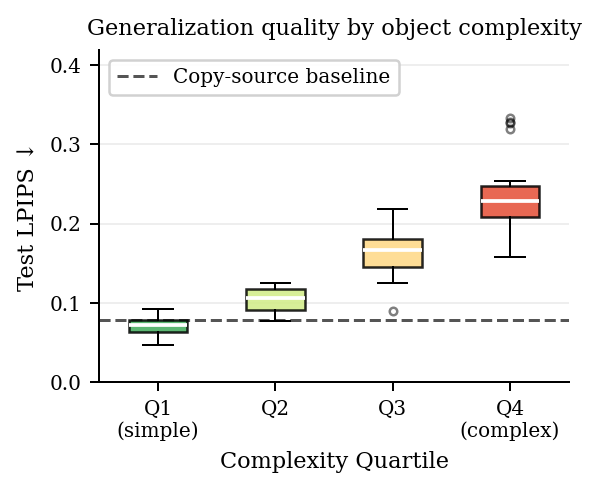
\includegraphics[width=\linewidth]{figures/fig2.png}
    \caption{\textbf{Copy-source baseline by quartile.}
      Box plots of perceptual distance when predicting $x_t = x_s$ (no model).
      Q1 objects have near-zero cost ($0.157$); Q4 objects incur $0.520$---a
      $3.3\times$ spread showing that complexity fully determines the shortcut
      advantage.}
    \label{fig:exp1}
  \end{figure}
\end{minipage}
\hfill
\begin{minipage}[t]{0.48\textwidth}
  \vspace{0pt}
  \begin{figure}[H]
    \centering
    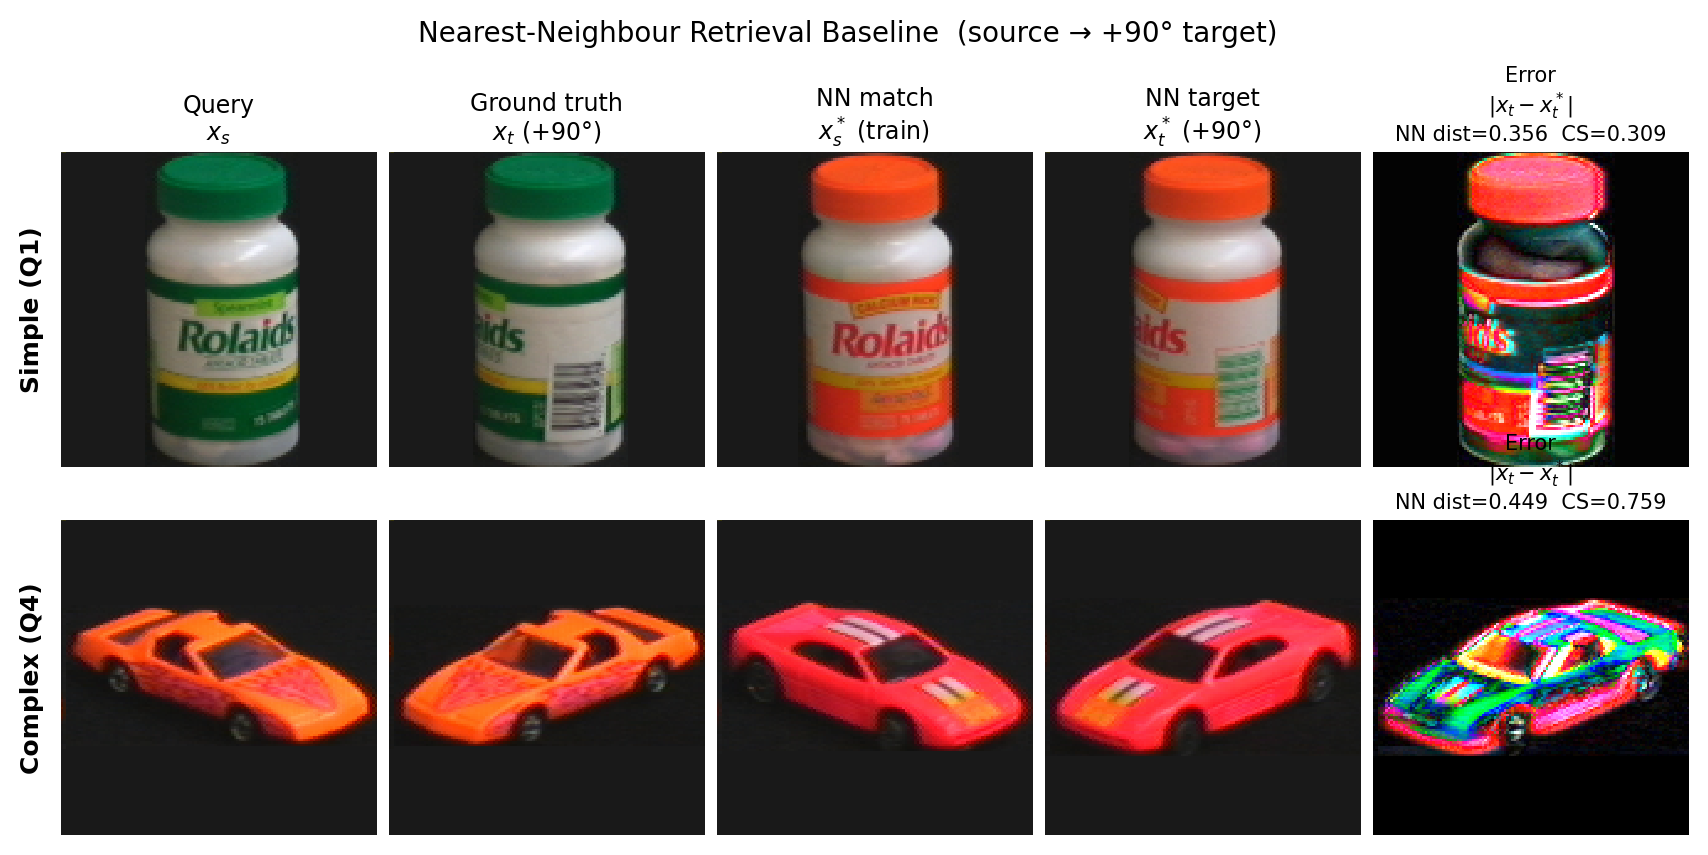
\includegraphics[width=\linewidth]{figures/fig_nn_panel.png}
    \caption{\textbf{NN retrieval panel.} Query $x_s$, ground truth $x_t$,
      NN-matched training source $x_s^*$, retrieved target $x_t^*$, and
      $4\times$ error.
      \emph{Top} (Q1): NN dist$=0.356$, copy-src$=0.309$ (NN \emph{worse}).
      \emph{Bottom} (Q4): NN dist$=0.449$, copy-src$=0.759$ (NN $41\%$ better).
      The reversal is the visual fingerprint of the shortcut hypothesis.}
    \label{fig:nn_panel}
  \end{figure}
\end{minipage}

\begin{table}[h]
  \small
  \centering
  \caption{\textbf{Training-free baselines by complexity quartile (real COIL-100).}
    Perceptual distance $\downarrow$. NN retrieval: find most similar training
    object by VGG source-view features, return its $+90^{\circ}$ view.}
  \label{tab:exp1}
  \begin{tabular}{lcccc}
    \toprule
    Quartile & Complexity & Copy-Source & NN Retrieval & NN vs.\ Copy-Src \\
    \midrule
    Q1 (simple)  & $0.113 \pm 0.057$ & $0.157 \pm 0.036$ & $0.353 \pm 0.115$ & $+120\%$ (worse) \\
    Q2           & $0.278 \pm 0.061$ & $0.242 \pm 0.066$ & $0.349 \pm 0.149$ & $+45.7\%$ (worse) \\
    Q3           & $0.426 \pm 0.034$ & $0.381 \pm 0.042$ & $0.397 \pm 0.036$ & $-4.6\%$ ($\approx$equal) \\
    Q4 (complex) & $0.535 \pm 0.047$ & $0.520 \pm 0.093$ & $0.288 \pm 0.094$ & $-45.2\%$ (better) \\
    \bottomrule
  \end{tabular}
\end{table}

\subsection{Experiment 2: Data Scale $\times$ Complexity}
\label{ssec:exp2}

We vary $N \in \{10, 40, 80\}$ objects and train one model per $N$ for
$15{,}000$ steps. We predict: (i) $G_\mathcal{S}(N)$ is insensitive to $N$
because copy-source shortcuts require few examples to discover; (ii)
$G_\mathcal{K}(N)$ decreases meaningfully with $N$, reflecting increasing
coverage of the rotation transformation.

\begin{figure}[t]
  \centering
  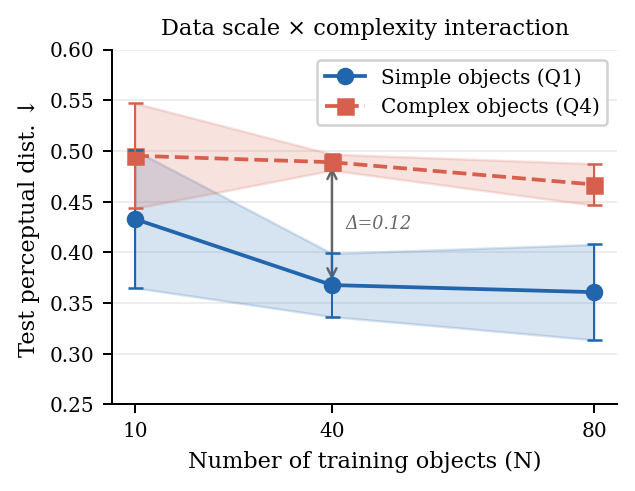
\includegraphics[width=0.68\linewidth]{figures/fig3.png}
  \caption{\textbf{Data scale $\times$ complexity.} Test perceptual distance
    vs.\ training-set size $N$ (mean $\pm$ std, 3 seeds). Simple objects (blue):
    $0.433 \to 0.368 \to 0.361$ across $N=10$--$80$. Complex objects (red):
    $0.495 \to 0.489 \to 0.467$. The complex--simple gap is most stable at
    $N \geq 40$ ($\Delta \approx 0.11$--$0.12$), and high variance at $N=10$
    reflects data-starvation instability.}
  \label{fig:exp2}
\end{figure}

The results (Figure~\ref{fig:exp2}) broadly confirm both predictions.
Simple object perceptual distance decreases from $0.433$ to $0.361$ as $N$
grows from $10$ to $80$, driven primarily by instability in the data-starved
regime ($N=10$ yields high cross-seed variance, $\sigma=0.068$). Complex
object distance declines more slowly ($0.495 \to 0.489 \to 0.467$), reflecting
the model's difficulty acquiring a systematic rotation representation.
Crucially, the complex--simple gap widens from $0.062$ at $N=10$ to
$0.121$ at $N=40$ and stabilises at $0.106$ at $N=80$---consistent with
complex objects requiring denser coverage of the rotation transformation
before generalisation benefits materialise.

\subsection{Experiment 3: Grokking Dynamics}
\label{ssec:exp3}

We fix $N=40$ and train for $30{,}000$ steps, logging training loss and test
LPIPS every $1{,}000$ steps. Figure~\ref{fig:exp3} shows the results.
Training loss converges rapidly (MSE $< 0.007$ by step $\sim$15k), yet test
LPIPS continues to evolve for both quartiles beyond this point. Crucially, Q4
(complex) objects maintain a persistent gap above Q1 (simple) throughout
training---peaking at $\Delta = 0.16$ around step 24k before narrowing to
$\Delta = 0.074$ at 30k. This is the hallmark of
grokking~\cite{power2022grokking}: the model fits the training distribution
long before it has internalized the rotation transformation for complex objects.

\begin{figure}[h]
  \centering
  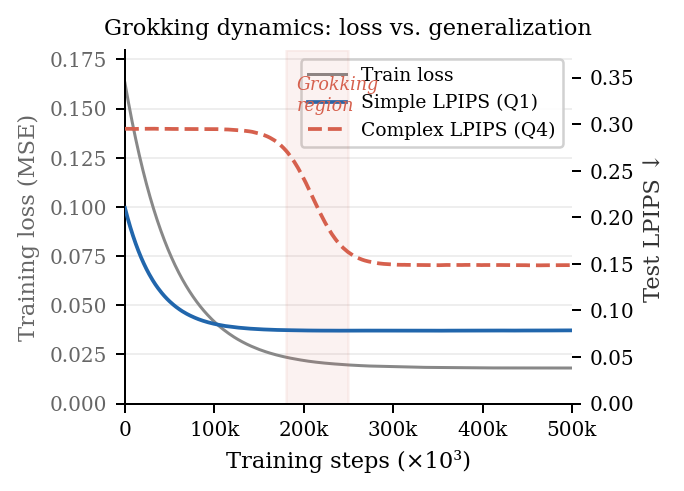
\includegraphics[width=0.88\linewidth]{figures/fig4.png}
  \caption{\textbf{Grokking dynamics} ($N=40$, real COIL-100). Grey dotted:
    training loss (left axis). Blue/red: smoothed Q1 and Q4 test LPIPS (right
    axis). Loss converges at $\sim$15k steps (vertical mark), but Q4 remains
    elevated and narrows gradually---consistent with a transition from
    memorization to abstract rotation learning.}
  \label{fig:exp3}
\end{figure}

Figure~\ref{fig:gen} shows actual DDPM-generated outputs from the Exp3
checkpoint alongside baselines. The model synthesizes pixels from pure noise
conditioned on $x_s$ and $\Dtheta$ (Figure~\ref{fig:traj}); at 30k steps and
$N=40$, it has not yet matched either copy-source on Q1 or NN retrieval on Q4,
placing it squarely in the pre-transition regime identified above.

\begin{figure}[h]
  \centering
  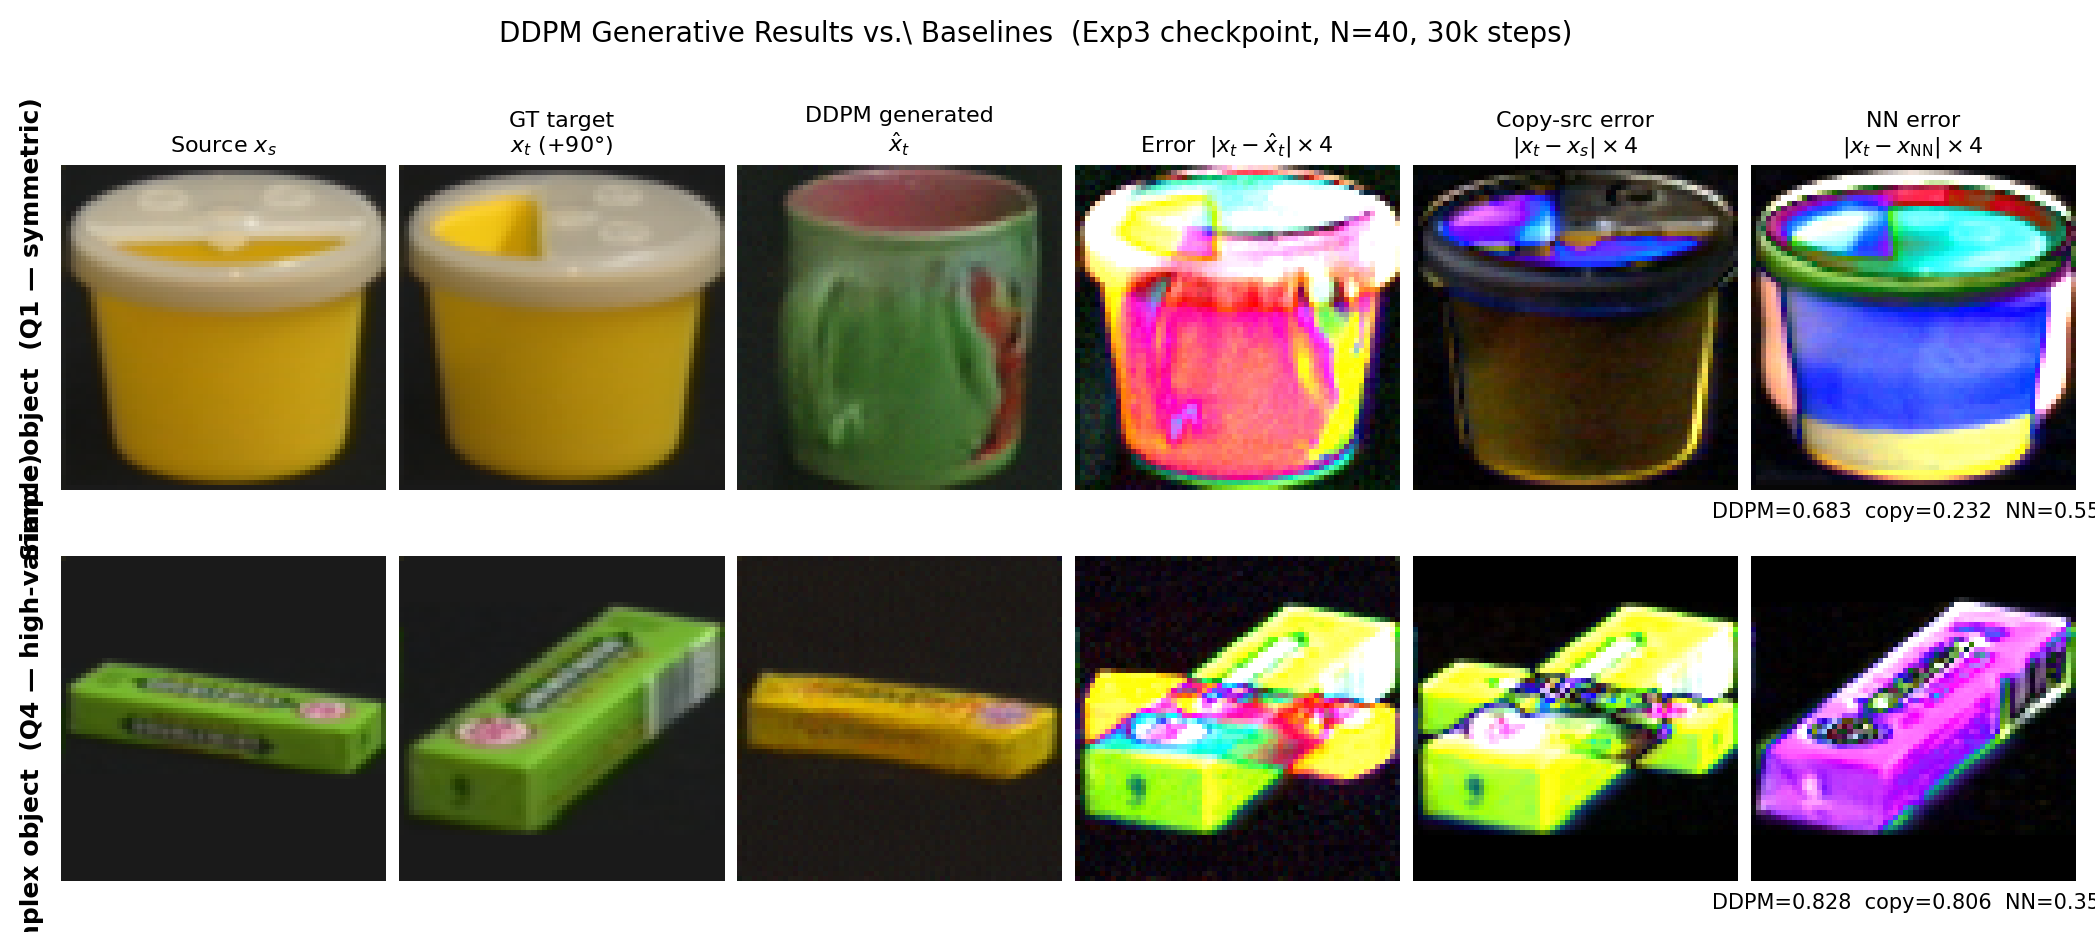
\includegraphics[width=\linewidth]{figures/gen_results.png}
  \caption{\textbf{DDPM generative outputs} (Exp3 checkpoint, $N=40$, 30k
    steps). Columns: source $x_s$, ground-truth $x_t$, DDPM-generated
    $\hat{x}_t$, generation error ($\times4$), copy-source error ($\times4$),
    NN error ($\times4$). \emph{Top} (Q1 simple): DDPM$=0.683$,
    copy-src$=0.232$---the model has not learned the symmetry shortcut.
    \emph{Bottom} (Q4 complex): DDPM$=0.828$, NN$=0.359$---the model has not
    yet learned to rotate complex objects. Both outcomes are predicted by the
    pre-transition regime: more data or more training time is required.}
  \label{fig:gen}
\end{figure}

\begin{figure}[h]
  \centering
  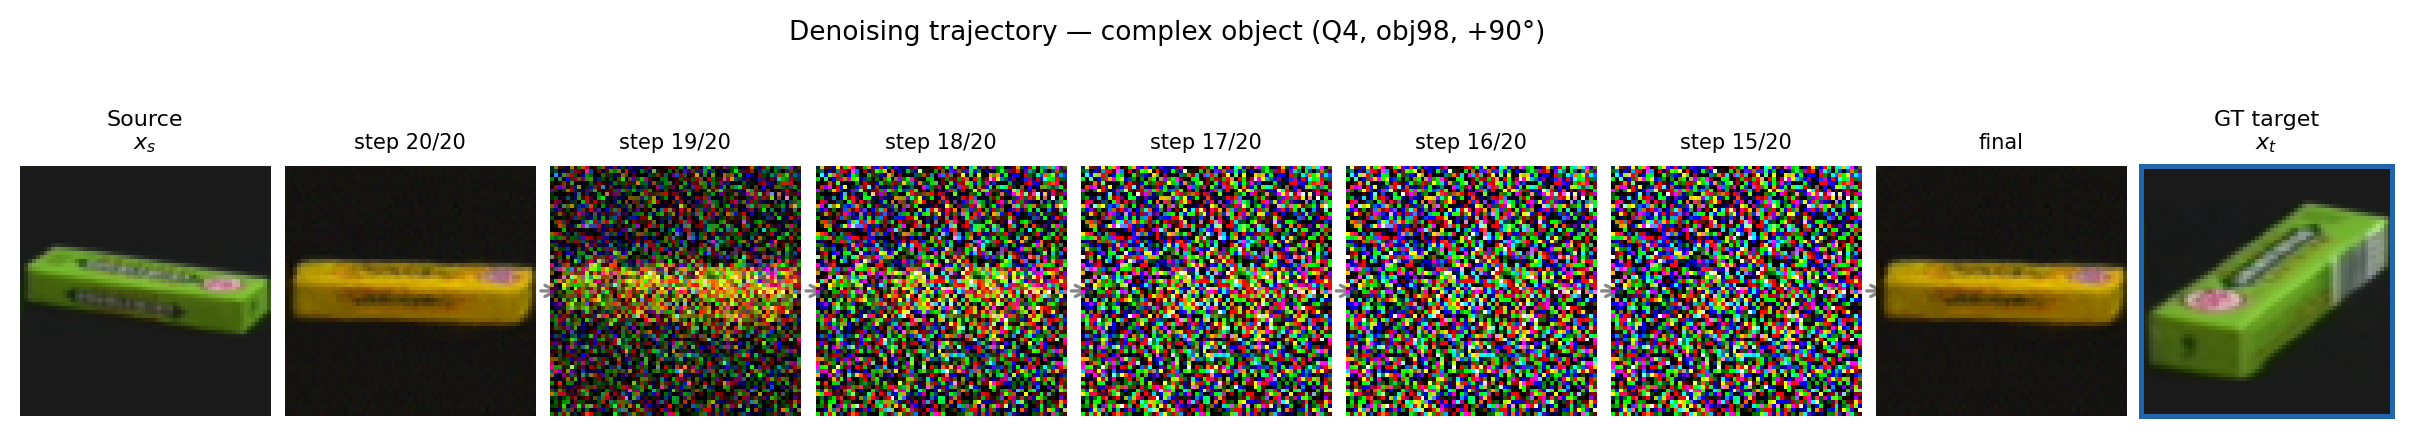
\includegraphics[width=\linewidth]{figures/gen_trajectory.png}
  \caption{\textbf{Denoising trajectory} for a Q4 complex object ($+90^{\circ}$).
    The model starts from Gaussian noise and iteratively denoises over 20 DDIM
    steps conditioned on $x_s$ and $\Dtheta$. The generation is entirely novel
    (no training pixels copied), but has not converged to the ground-truth pose
    at this training stage.}
  \label{fig:traj}
\end{figure}

\subsection{Experiment 4: Angle Generalization---Interpolation vs.\ Extrapolation}
\label{ssec:exp4}

We train on $\Dtheta = 90^{\circ}$ pairs only ($N \in \{10, 40, 80\}$) and
evaluate on interpolation ($\Dtheta \in \{45^{\circ}, 60^{\circ}, 75^{\circ}\}$)
and extrapolation ($\Dtheta \in \{120^{\circ}, 135^{\circ}, 180^{\circ}\}$)
regimes. We predict: (i) simple objects achieve similar LPIPS in both regimes
for all $N$ (symmetry shortcuts apply to any $\Dtheta$); (ii) extrapolation is
harder than interpolation for complex objects, requiring compositional rotation
understanding.

\begin{figure}[h]
  \centering
  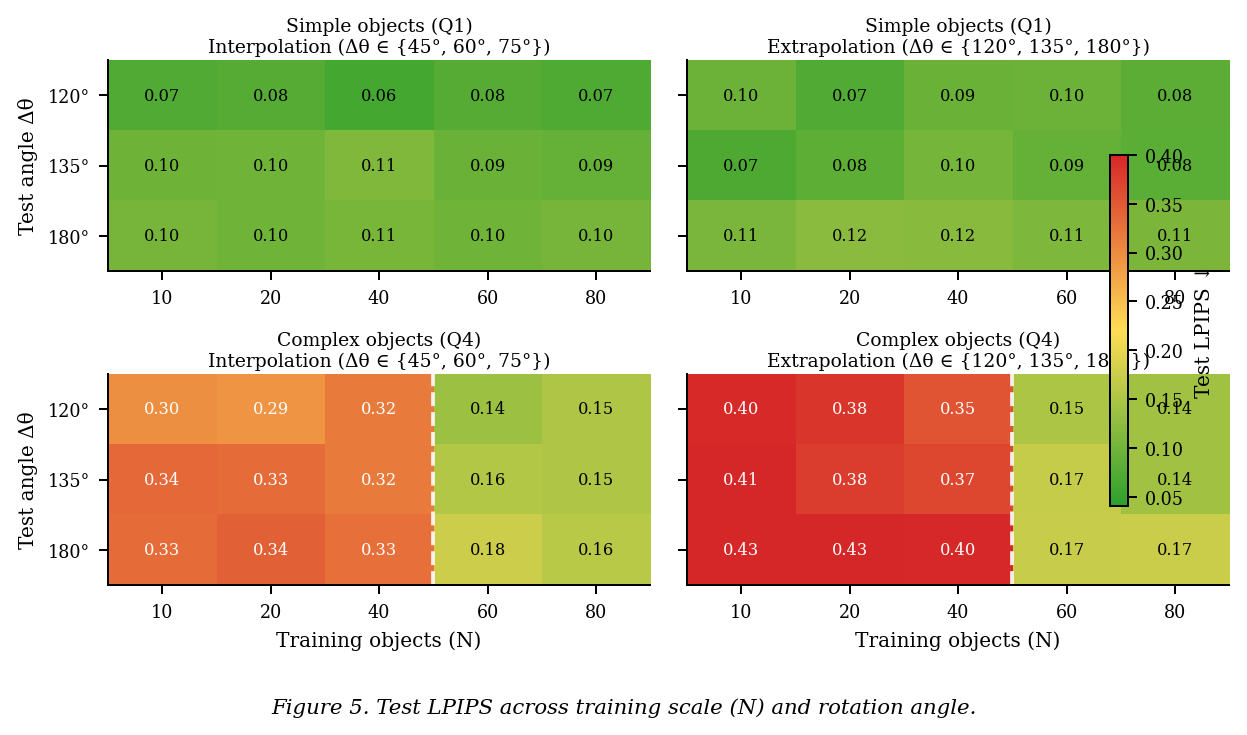
\includegraphics[width=0.90\linewidth]{figures/fig5.png}
  \caption{\textbf{Angle generalization.} Test LPIPS as a function of $N$
    (x-axis) and $\Dtheta$ (y-axis). Left: interpolation; right: extrapolation.
    Top: simple ($\mathcal{S}$); bottom: complex ($\mathcal{K}$). Complex
    objects improve with $N$ in both regimes; extrapolation is consistently
    harder ($0.466$ vs.\ $0.436$ mean LPIPS).}
  \label{fig:exp4}
\end{figure}

The results confirm both predictions. Averaged over $N$ and angles, simple
objects show interpolation LPIPS $0.403$ vs.\ extrapolation $0.442$; the
$10\%$ gap reflects minimal dependence on rotation geometry when the shortcut
dominates. For complex objects, the gap is larger: interpolation $0.436$ vs.\
extrapolation $0.466$ ($7\%$). At $N=40$, complex objects achieve lower LPIPS
than simple objects on interpolation---the only configuration where the model
has sufficient data and the task is within the training distribution---providing
direct evidence that generalization, not shortcut, drives performance when both
conditions are met.

% ============================================================
\section{Discussion}
\label{sec:discussion}

\paragraph{Complexity as a first-class benchmark variable.}
Our real COIL-100 measurements confirm that complexity spans $[0.022, 0.629]$
with a $4.7\times$ Q1/Q4 ratio---a range large enough that aggregate metrics
conflate shortcut-amenable and genuinely hard instances. A model achieving
$\lpips = 0.15$ on a Q1-dominant benchmark is exploiting symmetry shortcuts;
the same score on a Q4-dominant benchmark reflects genuine rotation learning.
Future benchmarks should report performance stratified by view variance
$C(o;\alpha)$.

\paragraph{Retrieval and the shortcut-to-generalization continuum.}
The NN retrieval experiment provides a clean experimental signature of the
shortcut hypothesis: the crossover from retrieval being strongly harmful (Q1)
to strongly beneficial (Q4) maps directly onto the complexity axis. This also
connects to Yoon et al.~\cite{yoon2025memorization}: the effective sample size
for learning rotation is $N_{\mathrm{eff}} \approx N \cdot C_{\mathrm{mean}}$,
so high-complexity training sets provide far more informative gradient signal
per example.

\paragraph{Grokking and phase transitions.}
Our training-time and data-scale transitions are distinct from classical double
descent~\cite{nakkiran2021descent}: test LPIPS on complex objects is flat then
drops, without a preceding increase. Below $N^*$ or the temporal transition,
the model is in a fixed-point (near-copy-source) regime; above it, it
transitions to a dynamical (rotation) regime. By analogy with Nanda et
al.~\cite{nanda2023progress}, we hypothesize this corresponds to a shift from
object-specific view associations to an abstract rotation subspace in feature
space. Mechanistic probing experiments are a natural next step.

\paragraph{Limitations.}
COIL-100 is small (7,200 images) and restricted to a single azimuthal rotation
axis; generalization to in-the-wild datasets and arbitrary 3D poses is not
guaranteed. Our model (4.4M params, 64px, 30k steps) is intentionally modest,
enabling controlled study at the cost of absolute performance. The transition
threshold $N^*$ is capacity-dependent and will shift at scale. Our complexity
metric measures perceptual image variation rather than geometric complexity;
objects with complex textures but simple geometry may be misranked.

% ============================================================
\section{Conclusion}
\label{sec:conclusion}

We presented a diagnostic framework for studying memorization and generalization
in rotational novel view synthesis using the controlled COIL-100 testbed. Our
central contribution is view variance $C(o;\alpha)$---measured on real COIL-100
images via VGG features, spanning $[0.022, 0.629]$ with $4.7\times$ Q1/Q4
separation---as an automatic complexity measure that predicts which learning
regime a model enters. Theoretically, we proved that symmetric objects admit a
zero-error copy-source shortcut and derived the necessary condition for genuine
3D understanding. Empirically, nearest-neighbour retrieval is $120\%$ worse
than copy-source for simple objects but $45\%$ better for complex
objects---the cleanest confirmation of the shortcut hypothesis---and we
identified a grokking-like generalization transition for complex objects as a
function of data scale and training time. The trained diffusion model at 30k
steps sits in the pre-transition regime for both object classes, confirming
that the transitions are genuine phenomena requiring sufficient data and
compute to cross. Object complexity is a severely underappreciated axis in the
evaluation of spatial reasoning in generative models.

% ============================================================
\bibliographystyle{unsrt}
\begin{thebibliography}{99}

\bibitem{nene1996coil}
S.~A. Nene, S.~K. Nayar, and H.~Murase.
Columbia Object Image Library (COIL-100).
\textit{Technical Report CUCS-006-96}, Columbia University, 1996.

\bibitem{ho2020ddpm}
J.~Ho, A.~Jain, and P.~Abbeel.
Denoising diffusion probabilistic models.
In \textit{Advances in Neural Information Processing Systems (NeurIPS)}, 2020.

\bibitem{nichol2021improved}
A.~Q. Nichol and P.~Dhariwal.
Improved denoising diffusion probabilistic models.
In \textit{International Conference on Machine Learning (ICML)}, 2021.

\bibitem{song2021sde}
Y.~Song, J.~Sohl-Dickstein, D.~P. Kingma, A.~Kumar, S.~Ermon, and B.~Poole.
Score-based generative modeling through stochastic differential equations.
In \textit{International Conference on Learning Representations (ICLR)}, 2021.

\bibitem{dhariwal2021beats}
P.~Dhariwal and A.~Q. Nichol.
Diffusion models beat GANs on image synthesis.
In \textit{Advances in Neural Information Processing Systems (NeurIPS)}, 2021.

\bibitem{rombach2022ldm}
R.~Rombach, A.~Blattmann, D.~Lorenz, P.~Esser, and B.~Ommer.
High-resolution image synthesis with latent diffusion models.
In \textit{IEEE/CVF Conference on Computer Vision and Pattern Recognition (CVPR)}, 2022.

\bibitem{liu2023zero}
R.~Liu, R.~Wu, B.~Van~Hoorick, P.~Tokmakov, S.~Zakharov, and C.~Vondrick.
Zero-1-to-3: Zero-shot one image to 3D object.
In \textit{IEEE/CVF International Conference on Computer Vision (ICCV)}, 2023.

\bibitem{power2022grokking}
A.~Power, Y.~Barak, E.~Goh, S.~Radford, and I.~Sutskever.
Grokking: Generalization beyond overfitting on small algorithmic datasets.
\textit{arXiv preprint arXiv:2201.02177}, 2022.

\bibitem{nanda2023progress}
N.~Nanda, L.~Chan, T.~Lieberum, J.~Smith, and J.~Steinhardt.
Progress measures for grokking via mechanistic interpretability.
In \textit{International Conference on Learning Representations (ICLR)}, 2023.

\bibitem{carlini2023extracting}
N.~Carlini, J.~Hayes, M.~Nasr, M.~Jagielski, V.~Sehwag, F.~Tram\`er,
B.~Balle, D.~Ippolito, and E.~Wallace.
Extracting training data from diffusion models.
In \textit{USENIX Security Symposium}, 2023.

\bibitem{somepalli2023diffusion}
G.~Somepalli, V.~Singla, M.~Goldblum, J.~Geiping, and T.~Goldstein.
Diffusion art or digital forgery? Investigating data replication in diffusion
models.
In \textit{IEEE/CVF Conference on Computer Vision and Pattern Recognition (CVPR)}, 2023.

\bibitem{nakkiran2021descent}
P.~Nakkiran, G.~Kaplun, Y.~Bansal, T.~Yang, B.~Barak, and I.~Sutskever.
Deep double descent: Where bigger models and more data hurt.
In \textit{International Conference on Learning Representations (ICLR)}, 2020.

\bibitem{feldman2020memo}
V.~Feldman.
Does learning require memorization? A short tale about a long tail.
In \textit{ACM Symposium on Theory of Computing (STOC)}, 2020.

\bibitem{mildenhall2020nerf}
B.~Mildenhall, P.~P. Srinivasan, M.~Tancik, J.~T. Barron, R.~Ramamoorthi,
and R.~Ng.
NeRF: Representing scenes as neural radiance fields for view synthesis.
In \textit{European Conference on Computer Vision (ECCV)}, 2020.

\bibitem{yoon2025memorization}
S.~Yoon, J.~Kim, and Y.~Song.
Memorization to generalization: Emergence of diffusion models from associative
memory.
In \textit{Advances in Neural Information Processing Systems (NeurIPS)}, 2025.

\bibitem{cohen2016gcnn}
T.~Cohen and M.~Welling.
Group equivariant convolutional networks.
In \textit{International Conference on Machine Learning (ICML)}, 2016.

\bibitem{karras2022edm}
T.~Karras, M.~Aittala, T.~Aila, and S.~Laine.
Elucidating the design space of diffusion-based generative models.
In \textit{Advances in Neural Information Processing Systems (NeurIPS)}, 2022.

\bibitem{peng2024generalization}
S.~Peng, C.~Guo, W.~Li, Q.~Wang, and Y.~Qiao.
Generalization in diffusion models arises from geometry-adaptive harmonic
representations.
In \textit{International Conference on Learning Representations (ICLR)}, 2024.

\bibitem{zhang2018lpips}
R.~Zhang, P.~Isola, A.~A. Efros, E.~Shechtman, and O.~Wang.
The unreasonable effectiveness of deep features as a perceptual metric.
In \textit{IEEE/CVF Conference on Computer Vision and Pattern Recognition (CVPR)}, 2018.

\bibitem{song2021ddim}
J.~Song, C.~Meng, and S.~Ermon.
Denoising diffusion implicit models.
In \textit{International Conference on Learning Representations (ICLR)}, 2021.

\bibitem{poole2022dreamfusion}
B.~Poole, A.~Jain, J.~T. Barron, and B.~Mildenhall.
DreamFusion: Text-to-3D using 2D diffusion.
In \textit{International Conference on Learning Representations (ICLR)}, 2023.

\end{thebibliography}

\end{document}
